\chapter{Theoretical background}
%PR 3 St 2. Some intro recap motivation
Our goal, is to add the final steps in the theory chain which transforms the GRMHD simulations into interferometric observables. For this to be achieved and for the theory higher up in the chain to be maximally useful in data interpretation, realistic signal corruptions need to be considered. Hence, the purpose of this module is to further the sophistication of the interplay between theory and observation in the field.
%The plan for the chapter? PR 3 St 2
The signal corruptions which we have identified as the most prominent occurs in the troposphere, interstellar medium (ISM) and within the stations themselves. First I will review some EM wave fundamental and introduce scattering theory, which is applicable to both the radiative process occuring in the troposphere and ISM. Following the general introduction I will explore each specific case.

\subsection{Radio Interferometry}
%PR 2 St 3 Define basic radio interferometry concepts. Reference Thompson, Smirnov

%Visibility, the interferometric measurement i.e. measuring electric field covariance (smirnov_1)
% Define the correlations measured

%UV Sampling, Earth rotation synthesis

% van-citterlike theorem a relationship between the image of the sky and it's fourier transform.

%\begin{equation}\label{eq:vis_im}
%van-citterlike theorem
%\end{equation}•

\subsubsection{Measurement Equation}
%PR 2 St 3, reference smirnov
%Follow Smirnov, first RIME paper , Introduce Jones formalism


%DDE vs DIE.. + diagram?

\subsubsection{mm-VLBI observables and data products}
%PR 2 St 2

%Visibility amplitudes, closure quantities, polarisation ratios, and images.
If the visibility phase is highly variable as in the case of a turbulent atmosphere,  conventional calibration and imaging techniques have severely limited (if any) success. However information can still be extracted from the raw visibilities in the form of closure quantities \citep{Monnier_2007} or polarisation ratios \citep{Fish_2009}. Closure phase, defined as the sum of 3 visibility phases of a triangle of stations $\left\{i,j,k\right\}$, is a probe of asymmetry in source structure,
\begin{equation}
\Phi_{ijk} = \phi_{ij}+\phi_{jk}+\phi_{ki}.
\end{equation}

\noindent Because most signal corruptions are station based, the gain phase terms $\phi_{ij}=\phi^{\rm true}+ \phi^G_i -\phi^G_j$ for each antenna will cancel, yielding a more robust observable. 

The uncertainty on the closure phase is model dependent \citep{Rogers_1995} and is given as a function of the SNR $s$ of each baseline 

\begin{equation}\label{eq:ucp}
u(\Phi_{ijk}) = \frac{\sqrt{4 + (s_{ij}s_{jk})^2 + (s_{jk}s_{ki})^2 + (s_{ij}s_{ki})^2 +
                        2(s_{ij}^2+s_{jk}^2+s_{ki}^2)}}{s_{ij}s_{jk}s_{ki}},
\end{equation}

\noindent where $s_{ij}$ is defined as
\begin{equation}
s_{ij}=|V_{ij}| \sqrt{\frac{ \tau \Delta \nu}{SEFD_i SEFD_j}},
\end{equation}
where $\tau$ is the vector averaging timescale, $\Delta \nu$ is the bandwidth, $|V_{ij}|$ is the visibility amplitude and $SEFD$ is the system equivalent flux density. The result that closure phase is entirely immune to station based effects breaks down however when time averaging in the presence of baseline dependent effects like thermal noise as illustrated in section~\ref{closure_errors}.
 
 \subsubsection{Variability and the static source assumption}
%PR 1 St 1

%the assumption and how it breaks the image-vis fourier transform relation
Implicit in our description of interferometry above, we assumed that the source remains approximately unchanged or static during the course of the observation. However, if this assumption does not hold (i.e. if the source is time-variable),  the visibilities measured over the course of an observation can no longer be related to a single image and if they are, the resulting image would appear smeared out as it is averaged over many realisations. 
%explicitly defining variability as any intrinsic source variability
Note that I am using the term `variability' in a general sense which refers to changes in any source observables. Most commonly variability is refers to changes in source flux (visibility amplitude) but I include changes in source structure and position (visibility phase) and source polarisation. Practically it is difficult to separate source and instrumental variability without accurate models and measurements for all non-source signal propagation effects. 
%Observed variability from SgrA
Although the static source assumption holds for most interferometric observations, the accretion flow and/or magnetic field structures around a SMBH can be variable on far shorter timescales. The primary mm-VLBI target, Sgr~$^\star$,  exhibits variability on timescales of minutes to hours in the radio (including in EHT observations), near-infrared (NIR), and X-ray bands \citep[e.g.][]{Baganoff_2001, Genzel_2003, Yusef-Zadeh_2006, Maronne_2006, Fish_2011, Johnson_2015b}. This wealth of observational data has yielded several answers but the origin of the variability is still highly debated. To explain the observed delays between flares in different frequency bands, an expanding adiabatic plasma model (Marrone, 2008) has been presented however a recent flare observed with the EHT did not exhibit the increase in size expected from an expanding plasma outflow model \cite{Fish_2011}.  Signatures of periodic variability at NIR and x-ray \citep{Genzel_2003; Belanger_2006} have been used to argue for the presence of orbiting hotspots \cite{Doeleman_2009}. As the Innermost Stable Circular Orbit (ISCO) depends on spin of the BH, the spin can be constrain through the detection periodic orbital features. However a longer light curve in the NIR is more representative of a power-law scale variability \cite{Meyer_2008}. These observations point to the possibility of multiple flaring mechanisms. An important mm-VLBI observational result is that variability in the polarisation domain is far more rapid than the total intensity (Johnson 2015b), indicating the presence of highly variable magnetic fields.
%Light crossing analysis
In principle, the variability timescale can be comparable to the period of the Innermost Stable Circular Orbit (ISCO), which for Sgr~A$^\star$, ranges from 4 minutes in the maximally rotating realisation to about half an hour for a non-rotating BH. The ISCO period for M87 is longer on the order of day scales. Considering light crossing times $\Delta t_{\rm cross}$, we can estimate the angular size $\theta$ of the emission region to be of order $\theta \sim \Delta t_{\rm cross} c /D_{\rm src}$, where c is the speed of light and $D_{\rm src}$ is the observer-source distance. Hence for Sgr~$^\star$ at a distance of $8.3$~kpc (Gillessen, 2009), for a flare of duration $ \Delta t_{\rm cross} =10$~min, which corresponds to scales of  $15 R_{\rm Sch}$, further evidence of emission areas close the event horizon.
%There are some ways to track/mitigate variability but this is beyond scope
If a flare is dominated by a localised variable structure, several approaches \citep{Doeleman_2009, Fish_2009b, Johnson_2014} show that EHT can track flaring structures with $\sim 5\ \mu$-arcsec precision using closure quantities and polarimetric ratios which could help map the spacetime around the BH. Alternatively \citet{Lu_2016} show that a gaussian weighting scheme can be applied to mitigate the effects of variability and measure the quiescent structure although approach would downweight the longest baselines. However all of these approaches assume only gaussian thermal noise, guassian-blurring in the ISM and no fringe-fitting errors.

\section{Signal Corruptions}

\subsection{Scattering basics}\label{sec:basic_scat}
%PR 1 St 1

%motivation
Millimetre wavelength radiation originating at the Galactic Centre is repeatedly scattered along the signal path to the Earth-based observer. The first occurrence is due to electron plasma in the interstellar medium (ISM) (\citealt{Bower_2006}, \citealt{Gwinn_2014}), while the second is due to poorly-mixed water vapour in the Earth's troposphere (\citealt*{Carilli_1999}, \citealt*{Lay_1997}). It is essential that the effects of the scattering phenomena are understood for a rigorous calibration and interpretation of data.  Towards this end, simulation modules approximating scattering in both media are implemented in \textsc{MeqSilhouette}. As an introduction to the separate descriptions of each, we review a simple scattering model.

%description of the model
An electro-magnetic wave is scattered when it passes through a medium with refractive index inhomogeneities. Following \citet{Narayan_1992}, this effect can be modeled as a thin screen, located between source and observer planes and orientated perpendicular to the line-of-sight. The screen, indexed by coordinate vector $\mathbf{x}$, adds a stochastic phase $\phi(\mathbf{x})$ to the incoming wave at each point on the screen, yielding a corrugated, outgoing wavefront. We define the Fresnel scale as  $r_{\rm F} = \sqrt{\lambda D_{\rm os}/2\pi}$, where $D_{\rm os}$ is the observer-scatterer distance, or the distance where the geometrical path difference $\frac{2\pi}{\lambda} (D_{\rm os} - \sqrt{D_{\rm os}^2 + r_{\rm F}^2}) =\frac{1}{2}$~rad.

%example calculation
To determine the resultant electric field at a point in the plane of the observer, indexed by coordinate vector $\mathbf{X}$, one has to take into account all possible ray paths from the screen to $\mathbf{X}$. To illustrate the model, a calculation of the scalar electric field generated by a point source, $\psi(\mathbf{X})$ yields the Fresnel-Kirchoff integral \citep*{BORN_1980}
\begin{equation}\label{Fresnel- Kirchoff}
\psi(\mathbf{X}) = C \int_{\rm screen} \exp\left[i\phi(\mathbf{x}) + i \frac{(\mathbf{x}-\mathbf{X})^2}{2 r_{\rm F}}\right]\mathbf{dx},
\end{equation}
where C is a numerical constant.

%define structure function
The statistics of $\phi(\mathbf{x})$ can be described by a power spectrum or equivalently the phase structure function,
\begin{equation}\label{eq:D_phi}
D_\phi (\mathbf{x},\mathbf{x'}) = < \left[ \phi(\mathbf{x} +\mathbf{x'}) - \phi(\mathbf{x})\right]^2 >,
\end{equation}
where $\mathbf{x}$ and $\mathbf{x'} $ represent two points on the screen and $<>$ denotes the ensemble average. 

There is evidence that $D_\phi$ can be reasonably approximated by a power law dependence on the absolute distance $r$ between points on the screen  \citep{Armstrong_1995,carilli_1997}
\begin{equation}
D_\phi (r) =  (r/r_0)^\beta,\qquad r^2 = \mathbf{x}^2 - \mathbf{x'}^2
\label{kolmogorov}
\end{equation}
where $r_{\rm 0}$ is the phase coherence length scale defined such that $D_\phi(r_{\rm 0}) = 1$~rad. 
%kolmogorov turbulence
Kolmogorov turbulence, which describes how kinetic energy injected at an outer length scale $r_{\rm out}$ cascades to increasingly smaller scales until finally dissipated at an inner length scale $r_{\rm in}$, predicts $\beta = 5/3$ in the domain ${r_{\rm in}<<r<<r_{\rm out}}$. This scaling has been demonstrated to be a reasonable approximation for the ISM over scales $r \sim 10^2$~km to $>1$~AU \citep*{Johnson_2015a}, and also for the troposphere with $r< \Delta h$, where $\Delta h$ is the thickness of the turbulent layer \cite{Coulman_1985}. The specifics of the tropospheric model will be explored further in later sections.

%Weak and strong
The two length scales, $r_{\rm F}$ and $r_{\rm 0}$, define the nature of the scattering which is split into the strong and weak regimes, Fig.~ref{fig:scatter}. In weak scattering, $ r_{\rm 0} \gg r_{\rm F}$ and hence by equation\ ~\ref{kolmogorov}, $D_{\phi}(r_{\rm F}) \ll 1$. This implies that most of the radiative power measured on a point $\mathbf{X}$ will originate from a screen area $A_{\rm weak} \approx \pi r_{\rm F}^2$. Whereas in the regime of \emph{strong scattering}, $ r_{\rm 0} \ll r_{\rm F}$ yielding  $D_{\phi}(r_{\rm F}) \gg 1$. This  results in coherent signal propagation onto the point $\mathbf{X}$ from multiple disconnected zones each of area $A_{strong} \approx \pi r_{\rm 0}^2$ \citep{Narayan_1992}. Scattering in the troposphere and ISM fall into the regimes of weak and strong scattering respectively.

%Weak and strong fig
\begin{figure*}
\begin{center}
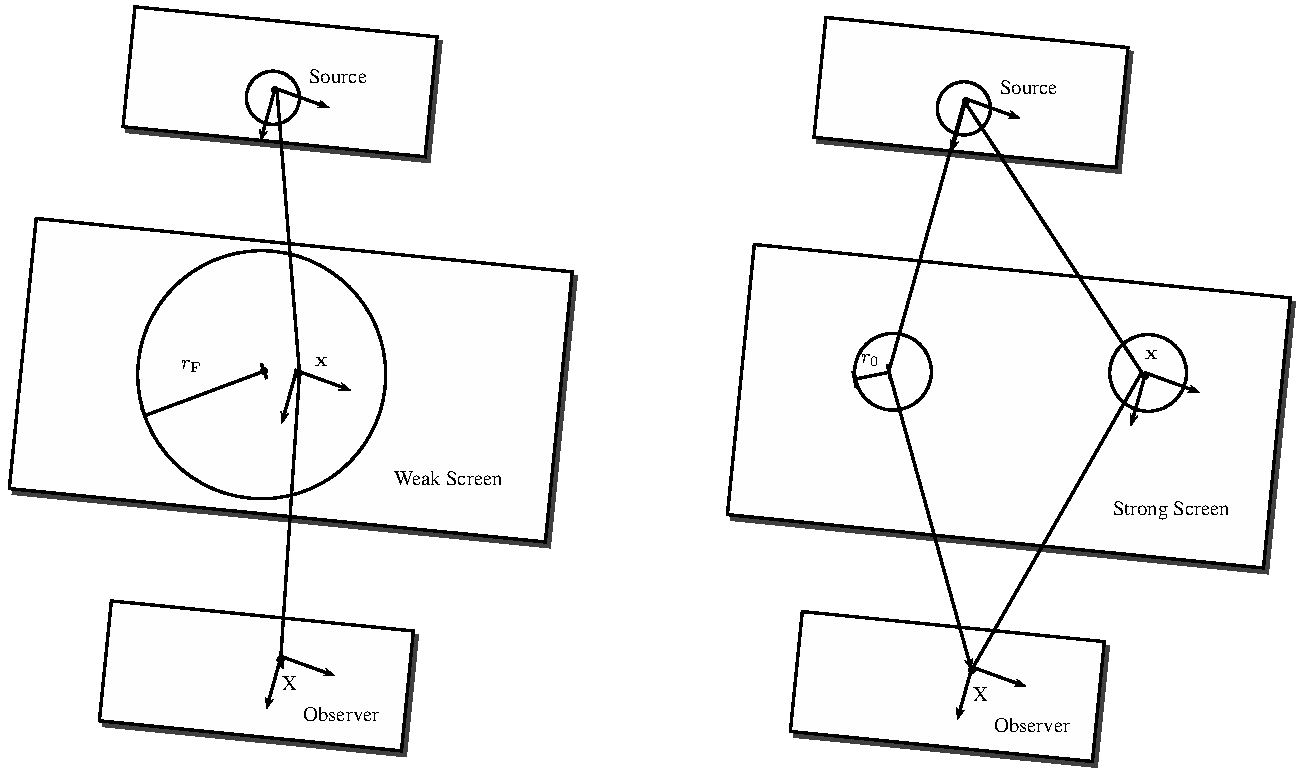
\includegraphics[width=1.\columnwidth]{Images/scatter.pdf}
\caption{Illustration depicting the basics of scattering in the weak (left) and strong (right) regimes. In the weak regime, the signal is coherently propagated over an area, $A_{\rm weak} \approx \pi r_{\rm F}^2$ whereas in the strong regime, coherent propagation is split over many areas of size $A_{strong} \approx \pi r_{\rm 0}^2$. \label{fig:scatter}
}
\end{center}
\end{figure*}

%frozen screen
To evolve the screen in time, we assume a frozen screen i.e. that the velocity of the individual turbulent eddies is dominated by the bulk motion of scattering medium \citep[e.g.][]{Lay_1997}. This allows us to treat the screen as frozen but advected over the observer by a constant motion. Hence time variability can be easily incorporated by the relative motion between source, scattering screen and observer.

\section{Interstellar medium scattering}
%PR 1 St 1.1 

%introduction and plan
Electron density inhomogeneities in the interstellar medium (ISM) plasma scatter the radio emission from the Galactic centre. Radio interferometric observations of Sgr~A$^\star$ have characterised the basic properties of the intervening plasma matrial, however extensive developments in scattering theory and simulations have proved essential to the interpretation of more subtle scattering phenomena. This section begins with the early observational results which studied the Gaussian blurring effect of the scattering; we then expand on the scattering theory introduced in Sec.~\ref{sec:basic_scat} to review the latest theoretical developments which explore the presence of scattering-induced substructure; finally we review recent observational results which account for scattering substructure in their data interpretation. 


%blurring
The dominant observational effect of the scattering for $\lambda \gtrsim$~cm is to convolve the intrinsic source structure with an elliptical Gaussian. The size of the Guassian exhibits a $\lambda^2$ scaling dependence over several orders of magnitude \citep[Fig.~\ref{fig:scattering_law}][]{Backer_1978, Shen_2005, Bower_2006, Lu_2011},which is consistent with the wavelength dependence of the refractive index of a plasma. In order to determine the parameters of the scattering kernel, i.e. major axis, minor axis and position angle,  one has to observe at wavelengths where the angular size of scattering ellipse is much larger than the expected source size. A Very Long Baseline Array (VLBA) + Green Bank Telescope (GBT) campaign \cite{Bower_2006} estimated the size at $1.31 \times 0.64$~mas cm$^{-2}$, oriented $78^\circ$ east of north. 


%debluring,uncertainties of the extrapolation
An accurate extrapolation of scattering kernel to 1.3~mm is important for the EHT scattering-mitigation strategy \cite{Fish_2014} which aims to deblur the scattered image through a deconvolution procedure. However as this extrapolation is over at least an order of magnitude, any small systematic error in the original measurement can significantly effect the 1.3~mm extrapolated parameters. A recent review of VLBI observations of Sgr~A$^\star$ \cite{Psaltis_2015} has noted that there are significant inconsistencies between different measurements. The authors used a Bayesian methodology to re-analyse the datasets resulting in increased uncertainties as shown in \ref{tab:ism_gauss}. The minor axis has a much larger uncertainty than the major axis due to the limited north-south coverage of the VLBA. 
%fig showing power laws of scattering and intrinsic source
\begin{figure*}
\begin{center}
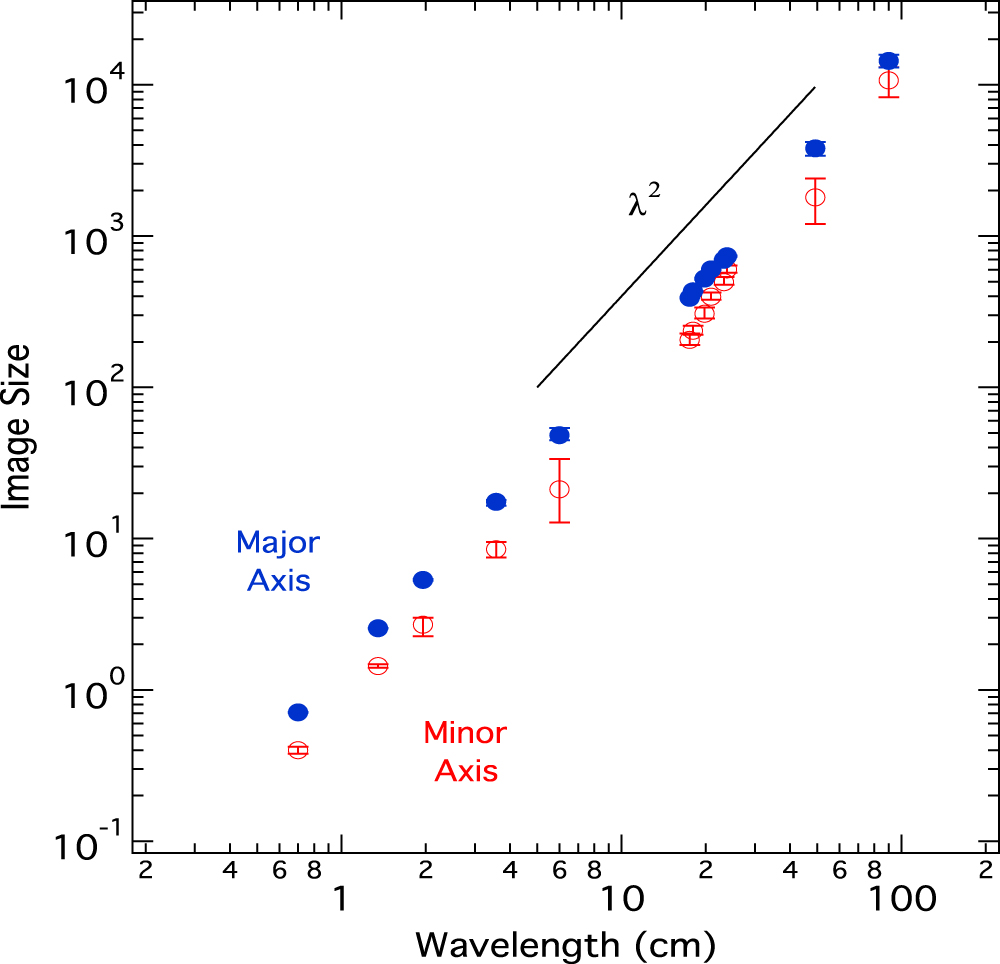
\includegraphics[width=0.6\columnwidth]{Images/scattering_law}
\caption{The $\lambda^2$ dependence of scattering kernel size is shown by the solid line. This has been derived from measurements made at $\lambda > 17$~cm \cite{Bower_2006}. The dotted line shows the derived intrinsic source size which scales as $\lambda^1.44$. This was derived from measurements in the wavelength range, 2~cm~$< \lambda < 1.3$~mm. The red circles show major-axis observed sizes of Sgr~A$^\star$  and the green points show the derived intrinsic major-axis size. This plot was reproduced from \citet{Doeleman_2008}.\label{fig:scattering_law}
}
\end{center}
\end{figure*}
%table showing latest scattering kernel parameters
\begin{table}[]
\centering
\caption{A re-analysis of VLBI observations of Sgr~A$^\star$ by \citet{Psaltis_2015} has yielded revised estimates of the parameters associated with the Gaussian scattering kernel. An accurate estimation is needed for accurate extrapolation to 1.3~mm. Note that the position angle is measured East of North. \label{tab:ism_gauss}}
\begin{tabular}{l|ll}
\hline
major axis FWHM (mas/cm$^-2$)& 1.32 & 0.04 \\
minor axis FWHM (mas/cm$^-2$)& 0.82 & 0.21 \\
position angle ($^\circ$)& 77.8 & 9.7\\  
\hline
\end{tabular}
\end{table}


%theory - refractive scale and size of blurred image
The Gaussian blurring effect can explained by the simple scattering model introduced in  Sec.~\ref{sec:basic_scat}. Recall, that in the strong scattering regime light is propagated from coherent patches with linear size $\sim r_0$. Each patch will emit light coherently into a single-slit diffraction cone of angular size $\theta_{\rm scatt} \sim \lambda /r_0$. An observer will hence be illuminated by many patches spanning $\theta_{\rm scatt}$, yielding a blurred and broadened image, with projected size on the screen equal to the \emph{refractive scale} 
$$r_{\rm ref} = \theta_{\rm scatt} D_{\rm os} = r_{\rm F}^2/r_0.$$
$r_{\rm ref}$ is the third fundamental length scale in the strong scattering regime and is associated with the refractive timescale,
$$t_{\rm ref} = r_{\rm ref}/v.$$
%calculating r_0 given \theta_scatt 
We can calculate $r_0$ given the FWHM of $\theta_{\rm scatt}$ through the more precise relation
\begin{equation}\label{eq:theta_scatt}
 \theta_{\rm scatt} = \frac{2\sqrt{2\ln{2}}}{2\pi} \lambda / r_0 (M+1)
\end{equation} 
where $M = D_{\rm os}/R$ is the magnification and $R$ is the source-screen distance. The magnification factor is a correction to the model introduced in Sec.~\ref{sec:basic_scat} when $R \sim \infty$ no longer holds and should be used when calculating distances in the observer plane \citep*{Goodman_1989}.
%Locating the scattering screen Bower 2014
The location of the scattering medium was originally thought to be quite close to Sgr~A$^\star$. However, observations of a newly discovered pulsar, SGR~J1745-29, indicate that the scattering screen is located at a distance $D_{\rm os} = 5.8 \pm 0.3$~kpc, within the Scutum spiral arm. Using Eq.~\ref{eq:theta_scatt} and the parameters given in table \ref{tab:ism_gauss}, we find that the major axis of the coherence length at 1.3~mm, $r_0 \approx 3136.67$~km.


%shift to looking at refractive effects,theory, 3 regimes of scattering
As the VLBI moves to higher frequencies, focus has shifted away from the well-studied Gaussian convolution effect of ISM scattering and onto the presence of stochastic scattering-induced substructure. To understand this phenomenon, we must first develop our conceptual framework. 

Strong scattering can be further subdivided into \emph{snapshot}, \emph{average} and \emph{ensemble-average} regimes \citep*{Narayan_1989,Goodman_1989}. To understand the different regimes, remember that for each point on the source, the observer sees emission from coherent patches of size $\sim r_0$ spanning $\sim r_{\rm ref}$. The diffraction cones from each of the patches will interfere, resulting in a multi-slit \emph{diffractive scintillation} pattern. 

%snapshot regime
In the \emph{snapshot regime}, a compact source is observed with a narrow bandwidth and over a short time integration. This yields a single realisation of the diffractive scintillation pattern. By averaging over many snapshots, diffractive scintillation is quenched. This occurs if the source size $\theta_{\rm src}$ is much larger than the diffractive scale $\theta_{\rm src} \gg r_0/R$; if the fractional bandwidth $\delta \nu/\nu$ is much larger than the decorrelation bandwidth $\delta \nu/\nu \gg \delta \nu_{\rm dc}/\nu \approx (r_0/r_{\rm F})^2$ \citep{Narayan_1992}; or if the integration time $t_{\rm int}$ is much larger the diffractive timescale $t_{\rm int} \gg t_{\rm 0} = r_0/v$, where $v$ is the relative velocity between screen, source and observer. This regime is hence only accessible through observations of compact objects like pulsars. On a side note, observations in this regime can be used to probe the source with angular resolution given by the $\sim \lambda /r_{\rm ref}$ \citep[e.g.][]{Gwinn_2012}. This is because the scattering screen is essentially a lens of size $\approx r_{\rm ref}$.

%average regime 
In the \emph{average regime}, diffractive scintillation has been averaged over, however there still exists scintillation over scales comparable to the size of the scattered image of a point source $\sim r_{\rm ref}$, termed \emph{refractive scintillation}. Phase fluctuations on this scale acts like a weak lens to focus or defocus the $\lambda/ r_0$ scale diffraction cones in the direction of the observer. For a point source this would lead to weak flux variations in the total flux \citep{Narayan_1992}. We will show later that refractive scintillation leads to the presence of substructure for a resolved scatter-broadened source. In contrast to diffractive scintillation, refractive scintillation is much more difficult to average over. Typically the refractive time scale $t_{\rm ref} = r_{\rm ref}/v$ is on the order of weeks to months for Sgr~A$^\star$; the fractional decorrelation bandwidth is on the order of unity $\delta \nu_{\rm dc}/\nu \sim 1$; and the source has to be much larger than the image of a scattered point source $\theta_{\rm src} \gg \theta_{\rm scatt}$. 

%ensemble average
In the \emph{ensemble-average regime}, both diffractive and refractive scintillation have been averaged over. It is in this regime when  the scattering is equivalent to Gaussian convolution which is deterministic and not time variable. 


%approximation of the scattered image by Johnson 2015
A recent theoretical work \citep*{Johnson_2015a} has derived a useful approximation of the resolved scattered image $I_{\rm ss}$ in the average regime,
\begin{equation}\label{eq:scatterbrane}
I_{\rm ss}(\mathbf{x}) \approx I_{\rm src}\left(\mathbf{x} + r_{\rm F}^2 \nabla \phi(\mathbf{x})\right),
\end{equation}
where $\nabla$ is the directional derivative. Here we have used the same two-dimensional coordinate system, indexed by $\mathbf{x}$ to describe the source, screen and observer planes which are considered to be aligned along the vertical axis. The scattered image $I_{\rm ss}$ is approximated by a 'reshuffling' of the source image $I_{\rm src}$. As $|\nabla\phi| \sim 1/r_0$, the magnitude of the translation of points on $I_{\rm src}$ $\sim r_{\rm ref} \sim 10\ \mu$-arcsec in the case of Sgr~A$^\star$. 

%Coherence of the phase slope
Even though $\phi(\mathbf{x})$ is only coherent to $\sim r_{\rm 0}$, the directional phase derivative $\nabla \phi(\mathbf{x})$ remains spatially coherent over much larger scales. Following \citet*{Johnson_2015a}, the autocovariance of phase derivative can be related to the structure function
\begin{align}
\langle [ \partial_x \phi(\mathbf{x_0})] [ \partial_x \phi(\mathbf{x_0}+\mathbf{x})] \rangle &=\
-\partial^2_x \langle \phi(\mathbf{x_0}) \phi(\mathbf{x_0}+\mathbf{x}) \rangle \\
&= \partial_x^2 D_\phi(\mathbf{x}).
\end{align}

as $\langle \phi(\mathbf{x})^2 \rangle = 0$

Using a typical structure function \citep{johnson_dissertation},We are interested in the case $r_{\rm in} \gg r_0$, the structure function becomes \citep{johnson_dissertation}
\begin{equation*}
D_\phi =
\begin{cases}
\left( \frac{r}{r_0}\right)^2 & \text{if } r \ll r_{\rm in},\\
\frac{2}{\beta}\left( \frac{r_{\rm in}}{r_0}\right)^{2-\beta} \left( \frac{r}{r_0}\right)^\beta & \text{if } r \gg r_{\rm in}.
\end{cases}
\end{equation*}

Note that the structure function is quadratic at small scales as fluctuations are smooth andthen kolmogorov then constant (Tatarskii, 1971).
Hence We are interested in the case $r /gg r_{\rm in}$
\begin{equation}
\partial_x^2 D_\phi(\mathbf{x})= \left(\frac{r_{\rm in}}{r_0}\right)^{2-\beta}  2(\beta -1)  \frac{r^{\beta-2}}{r_0^\beta}
\end{equation}

Therefore in the Kolmogorov regime $\beta = 5/3$, the coherence of image shift relative to the refractive scale $\propto (r/r_0)^{-1/3}$. Inner scale extends coherence and outer scale cuts it off.

%ESTIMATE OF COHERENCE .. awaiting discussion with roger 

If $\nabla \phi(\mathbf{x})$ was incoherent between patches of size $\sim r_0$, this would effectively be convolution with Gaussian of size $r_{\rm ref}$. 
)

%Observations of substructure

A recent observation of Sgr~A$^\star$ at 3.5~mm by the VLBA+LMT \citep[see Fig.~ref{fig:substructure2}][]{Ortiz_2016} show that the closure phase measured is consistent with refractive scintillation. Another observation at 1.3~cm shows flux modulation due to scattering substructure $\sim 10$~mJy \citep{Gwinn_2014} and other predictions show $\sim 60$~mJy for long East-West baselines and $\sim 25$~mJy for long North-South baselines \citep*{Johnson_2015a}, assuming a Gaussian source of $FWHM=40\ \mu$-arcsec.

\begin{figure*}
\begin{center}
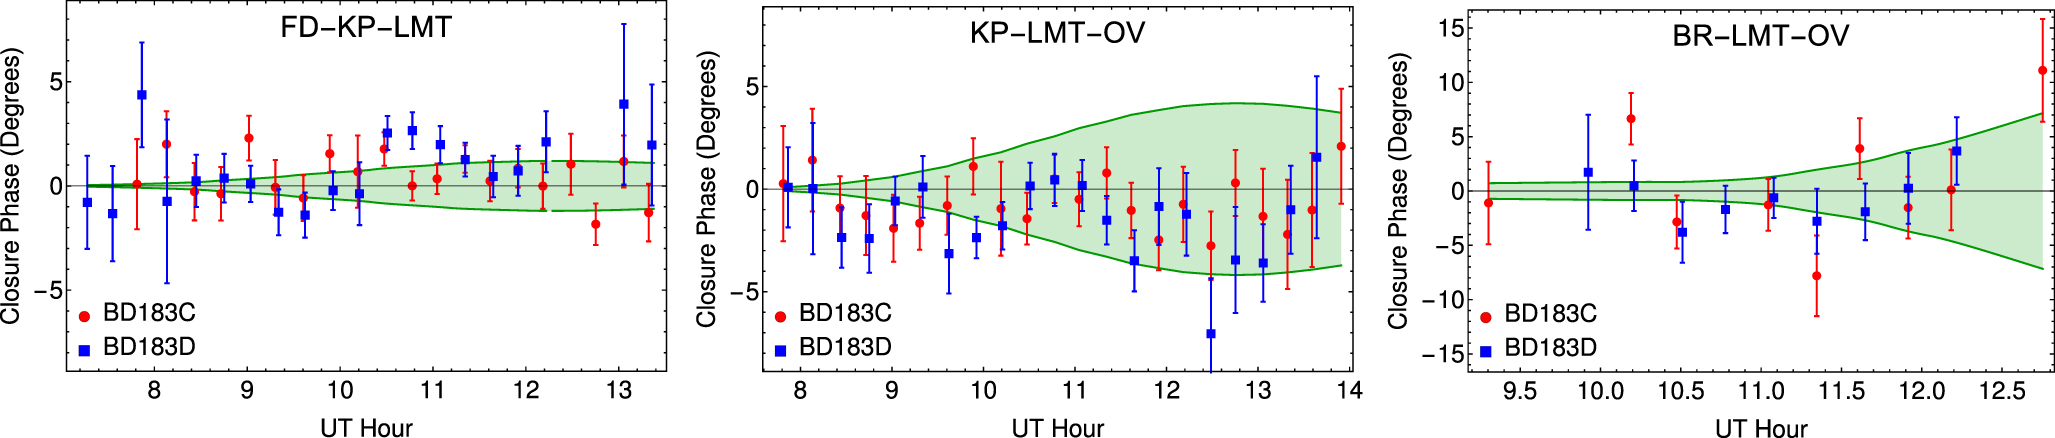
\includegraphics[width=\columnwidth]{Images/ism_cp}
\caption{Closure phases recorded in a VLBA + LMT observation of  Sgr~A$^\star$ at $\lambda = 3.5$~mm \cite{Ortiz_2016}. The data points are shown as red circles and blue squares and are only distinguished by the calibrator used. The green envelopes show the $1\sigma$ closure phase prediction induced by scattering-induced substructure. Reproduced from \citet{Ortiz_2016} \label{fig:substructure2}
}
\end{center}
\end{figure*}


%Distinguishing intrinsic source structure and variability
Distinguishing intrinsic source structure and variability and ISM variability is an interesting challenge. Observations at mm-wavelengths have revealed deviations from the $\lambda^2$ scattering scaling law, see Fig.~\ref{fig:scattering_law}. This is interpreted as due to the presence of intrinsic source structure and has been fitted with a power-law with an exponent of $1.34 \pm 0.01$ \cite{Lu_2011}. This has enabled the constraint of various theoretical models \cite{Bower_2006}, excluding advection-dominated accretion flows (ADAF) \cite{Narayan_1998} and Bondi-Hoyle accretion \cite{Melia_1994}. However observations extending over month timescales are required to properly sample the larger scale inhomogeneities and even with multiple epoch observations, it can be difficult to distinguish source and scattering characteristics \citep*{Macquart_2006}.

Knowledge of the scattering characteristics can allow the two to be decoupled without sampling a refractive ensemble. It therefore provides
a robust and rapid mechanism for quantifying refractive effects.



\section{Troposphere}
%PR 1 St 2

%Intro, typical temp, pressure, composition
The coherence and intensity of millimetre wavelength electromagnetic waves are most severely deteriorated in the lowest atmospheric layer, the troposphere, which extends up to an altitude of $7-10$~km above sea level and down to a temperature $T \sim 218$~K \citep{Thompson_2001}. The troposphere is composed of primary gases $\rm N_2$ and  $\rm O_2$, trace gases e.g. water vapour and $\rm CO_2$, as well as particulates of water droplets and dust. 
%section layout
We will first review basic propagation theory, then develop a theoretical a more sophisticated framework 



%propagation fundamentals and the relationship between delay-absorption-noise

Considering a quasi-monochromatic wave passing through a linear medium,
\begin{equation}
E(x,t) = E_0 \exp^{i(knx - 2\pi\nu t)},
\end{equation}		
where k is the propagation constant in free space equal to $2\pi \nu/c$ and $n$ is the complex index of refraction, $n= n_R + j n_I$. If $n_I$ is nonzero the wave will decay exponentially. The linear absorption coefficient or fraction of power absorbed per unit length traversing the medium is defined as 
\begin{equation}
\kappa_\nu = 4\pi \nu n_I/c.
\end{equation}
~\\
The phase velocity of light slows according to the refractive index, $v_p = c/n_R$, which results in a time delay.  Because the electric field is causal, $n_R$ and $n_I$ contain the same information and can be interchanged via the Kramers-Kronig relations. The time delay, $\delta t$ and optical depth $\tau$ can be calculated in general,
\begin{equation}\label{timedelay}
\delta t + i \tau =1/c \int_{medium} d^3\mathbf{x}\  (n(\mathbf{x}, \nu) -1),
\end{equation}
where the integral is over the total path through the medium.
~\\
Absorption is accompanied by emission and for a medium in local thermodynamic equilibrium, Kirchoff's law states that 
\begin{equation}\label{kirchoff}
\frac{\epsilon_\nu}{\kappa_\nu}=B_\nu(T),
\end{equation}
where $\epsilon_\nu = dI_\nu/dx$ is the macroscopic emission coefficient and $B_\nu(T)$ is the Planck function. Hence the absorbing molecules are also emitters, increasing system noise.\\

%Separate into average and turbulent - or maybe just consider radiative transfer in a static medium

\subsection{Average atmosphere}
%St 2

%Radiative transfer, how solving it will give observables in a self-consistent manner

We start from the unpolarised radiative transfer equation, which is unidirectional in the absence of scattering,
\begin{equation}
\frac{dI_\nu (s) }{ds} = \epsilon_\nu(s) -\kappa_\nu(s)  I_\nu (s),
\end{equation}\label{eq:rad_trans}
where $s$ is the coordinate along the signal path through the atmosphere, $I_\nu(s)$ is the specific intensity, $\epsilon_\nu$ is the macroscopic emission coefficient and $\kappa_\nu$ is the macroscopic absorption coefficient.  The assumption of local thermodynamic equilibrium (LTE) holds as the collisional timescale is much smaller than the time for spontaneous emission up to altitudes $\ge 80$ km after which there is only $\sim 0.001\%$ of mass left. (Pardo et al., ibid) Using Kirchoff's law, equation \ref{kirchoff}, multiplying by $\exp(-\tau_\nu)$ and integrating yields, 
\begin{equation}
I_\nu(s) = I_\nu(0) e^{-\tau_\nu (0,s) }+ \int_0^s B_\nu(s')e^{-\tau_\nu (s',s) }\kappa_\nu(s')ds'
\end{equation}
where  s' is a dummy variable in the same direction as s and $\tau_\nu (0,s) = \int_0^{s} k_\nu(s')ds'$. $I_\nu(0)$ is taken as the radiance from the cosmic background.\\
The above equation will allow us to calculate the noise temperature of the atmosphere by converting the output radiance at the ground $I_\nu(s)$ to  the equivalent blackbody temperature through inversion the Planck function. To calculate the opacity and complete the above integral, $\kappa_\nu$ needs to be calculated over the frequency range. Note again that  $\epsilon$ can easily be calculated from $\kappa$, and vice-versa, using Kirchoff's law.  The mean time delay can be calculated using the Kramers-Kronig relations. The fluctuations in time delay will be given in section \ref{turb} .

%properties of kappa_nu, absorption in the GHz regime
The absorption spectrum in the GHz range (e.g. \citealt{Pardo_2001}) is dominated by several transitions of $\rm H_2O$ and $\rm O_2$ as well as a pseudo-continuum opacity which increases with frequency. The pseudo-continuum opacity is due to the far wings of a multitude of broadened water vapour lines above 1~THz \citep{Carilli_1999}. 


%deriving the absorption coefficient
A general equation of the absorption coefficient for a transition between a lower $l$ and upper $u$ states is given in the original paper. Here we merely point out that it should be proportional to the energy of the photon, $h\nu_{l \to u}$, the transition probability or Einstein coefficient, $ B_{l \to u}$, the line-shape, $f(\nu,\nu_{l \to u})$ and the number densities $N$ of electronic populations. Line profiles which describe pressure broadening (perturbations to the Hamiltonian due to the presence of nearby molecules) and Doppler broadening are used. The condition of detailed balance further requires that decays from the upper state are included yielding, $g_u B_{u \to l} =g_l B_{l \to u}$, where $g$ is the degeneracy of the electronic state. Putting this together we find,

\begin{equation}
\kappa(\nu) _{l \to u}  \propto  h\nu   B_{l \to u}  \left(\frac{N_l}{g_l}  -  \frac{N_u}{g_u} \right) f(\nu,\nu_{l \to u}),
\end{equation}

\noindent where the Einstein coefficients are calculated from the inner product of the initial and final states with the dipole transition operator. The number densities of the two states, $N_u$ and $N_l$ in local thermodynamic equilibrium (LTE) are simply related to the local number density and temperature via Boltzmann statistics.

Assuming LTE, the electron population energy level  depends only on the local temperature, $T(s)$ and density of the \emph{i}th species $N_i(s)$. To perform the numerical integration, the atmosphere is discretised into layers of variable thickness with an accuracy $\sim0.1$ K. Temperature \& density profiles are calculated based on several station dependent inputs to the API, namely, ground temperature \& pressure, precipital water vapor content (PWV), altitude scale height of water vapour and the troposphere lapse rate.\\
~\\
Radiative transfer is applied to each absorption line through a sum over each atmospheric layer, chemical species and transition line, 
\begin{equation}
\tau_\nu = \sum_{i(layers)} \left[ \sum_{j(molec.)} \left( \sum_{k(lines)} \kappa_{\nu, k} \right)_j \right]_i \cdot \Delta s_i
\end{equation}
where $\Delta s_i$ is the path through the homogenous ith layer.\\
~\\
A general equation of the absorption coefficient for an arbitrary line transition $\kappa(\nu) _{l \to u}$ is given in the original paper. Here I merely note that it is proportional to the energy of the photon, $h\nu_{l \to u}$, the transition probability or Einstein coefficient, $ B_{l \to u}$ and the lineshape, $f(\nu,\nu_{l \to u})$. The condition of detailed balance requires that decays from the upper state are included yielding, $g_u B_{u \to l} =g_l B_{l \to u}$. Putting this together we have the proportionality,
\begin{equation}
\kappa(\nu) _{l \to u} \propto h\nu  B_{l \to u}  \left(\frac{N_l}{g_l}  -  \frac{N_u}{g_u} \right) f(\nu,\nu_{l \to u}).
\end{equation}
Physically, the lineshape originates from perturbations to the hamiltonian due to proximity to neighbouring molecules, called pressure broadening, and at lower pressures, thermal doppler broadening. A Van Vleck -Weisskopf (VVW) profile is used for pressure broadening. At lower pressures this is convolved with a gaussian which arises from the Maxwellian distribution. The population densities in LTE are given by boltzmann distribution
\begin{equation}
\frac{N_n}{N} = g_n \frac {\exp{-\frac{E_n}{kT}}}{Q}
\end{equation}
where Q is the partition function. $Q = \sum_i g_i  \exp{-E_n/kT}$. The Einstein absorption coeffients are calculated using 
\begin{equation}\label{coefficient}
B_{l \to u} = \frac{2\pi}{3\hbar^2} |<u|\mu|l>|^2,
\end{equation}
where $|u>$, $|l>$,$|\mu>$ are the wavefunctions of upper and lower states and the dipole transition operator respectively. \\
~\\
Transition lines at radio wavelengths result from rotational state transitions.  To calculate the inner product given in equation \ref{coefficient}, hamiltonians for linearly  symmetric rotors (e.g. $O_2$, $CO$) and asymetric rotors are used. The asymetric rotations are decomposed into three principal rotation axes with differing rotational constants governing each axis. Rotational constants were measured by the authors as well as drawn from a variety of literature. Partition functions and transition probability are calculated using approximations taken from the literature.\\
~\\
Far wing broadening of $H_2O$ lines $> 1.2$ THz extends to lower frequencies and is not completely represented by the VVW profile. This is believed to be due to self-self collisions of water molecules. Additionally there are terms from the dry atmosphere related to transient dipoles and Debye absorption which are not represented in the lineshape. To correct for these effects two pseudocontina are used. This takes the form of a power law dependence on $\nu$,$T$, and the molecular densities. The parameters involved in the pseudocontina as well as a subset of the rotational constants are based on Fourier transform spectroscopy measurements on Mauna Kea which was used to refine and test the model.\\
 ~\\

\subsection{Turbulent atmosphere} 
%PR 1 St 2

%phase variability in the GHz regime. 
%screen fig
In contrast to the other atmospheric chemical components, water vapour mixes poorly and its time-variable spatial distribution induces rapid fluctuations in the measured visibility phase at short wavelengths. The water vapour column density is measured as the depth of the column when converted to the liquid phase and is referred to as the precipitable water vapour (PWV). The PWV is, via the real component of the refractive index, directly proportional to phase offset, 
\begin{equation}
\delta\phi \approx \frac{12.6\pi}{\lambda} \times w, 
\end{equation}\label{eq:phi-pwv}

\noindent where $w$ is the depth of the PWV column \citep*{Carilli_1999} and an atmospheric temperature $T=270$~K has been assumed. This relationship between phase and water vapour content has been experimentally verified \cite{hogg_1981}. At 230~GHz, the change in PWV needed to offset the phase by 1~rad is $\Delta w\approx0.03$~mm. This sensitive dependence of phase coherence on atmospheric stability is aggravated by typically low antenna observation elevation angles, uncorrelated atmospheric variations between stations, and observing with a sparse VLBI array.

%How phase fluctuations pose a calibration challenge

Visibility phase instability  $\delta \phi(t)$ due to tropospheric turbulence is a fundamental limitation to producing high fidelity, science-quality maps with a mm-VLBI array \citep{Thompson_2001}. The coherence time-scale is typically too rapid ($\lesssim10$~s) for fast switching calibration, so other calibration procedures (e.g. water vapour radiometry, paired antennas, sub-arrays, and/or self-calibration) must be used. Self-calibration is the most commonly used but is limited by the integration time needed to obtain adequate SNR to fringe fit. This often leads to the use of closure quantities to perform model fitting (\citealt{Doeleman_2001}; \citealt{Fish_2011}).

The shifting distribution of water vapour in the troposphere causes the refractive index and hence the phase velocity to change on timescales of seconds and of spatial scales of metres (Thompson et al., ibid).  At centimeter wavelengths and below, water vapour in the troposphere dominates errors in delay and delay rate over hydrogen maser clock errors (Rogers \& Moran,1981). Stochastic phase errors lead to a decrease in flux due to incoherent vector averaging. This makes it difficult to obtain adequate SNR for calibration. The uncertainty in the phase degrades structural information which makes conventional imaging difficult and hence closure quantities are often used (e.g. Fish et al 2011). Incoherent phases represent a fundamental limit to all types of interferometry. 
Figure \ref{screen} gives a cartoon illustration of the shifting distribution of water vapour above a baseline. 
\begin{figure}[h!]
\centering
    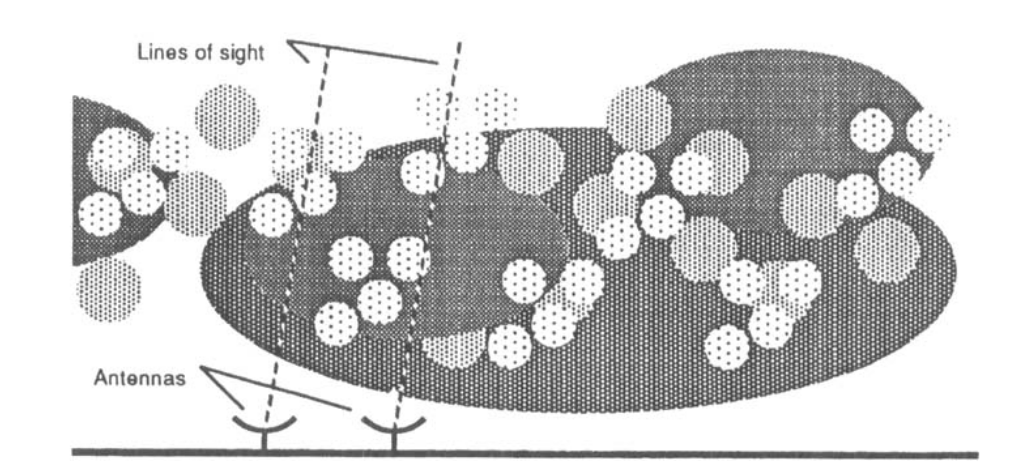
\includegraphics[height=60mm,width=120mm]{Images/screen}
    \caption{A cartoon illustration of poorly mixed water vapour moving over a baseline (credit : Thompson et al, ibid) \label{phase:screen}}
\end{figure}

%Following from basics scattering.. 


%carilli fig


%the different power law regimes


\begin{figure}[h!]
\centering
    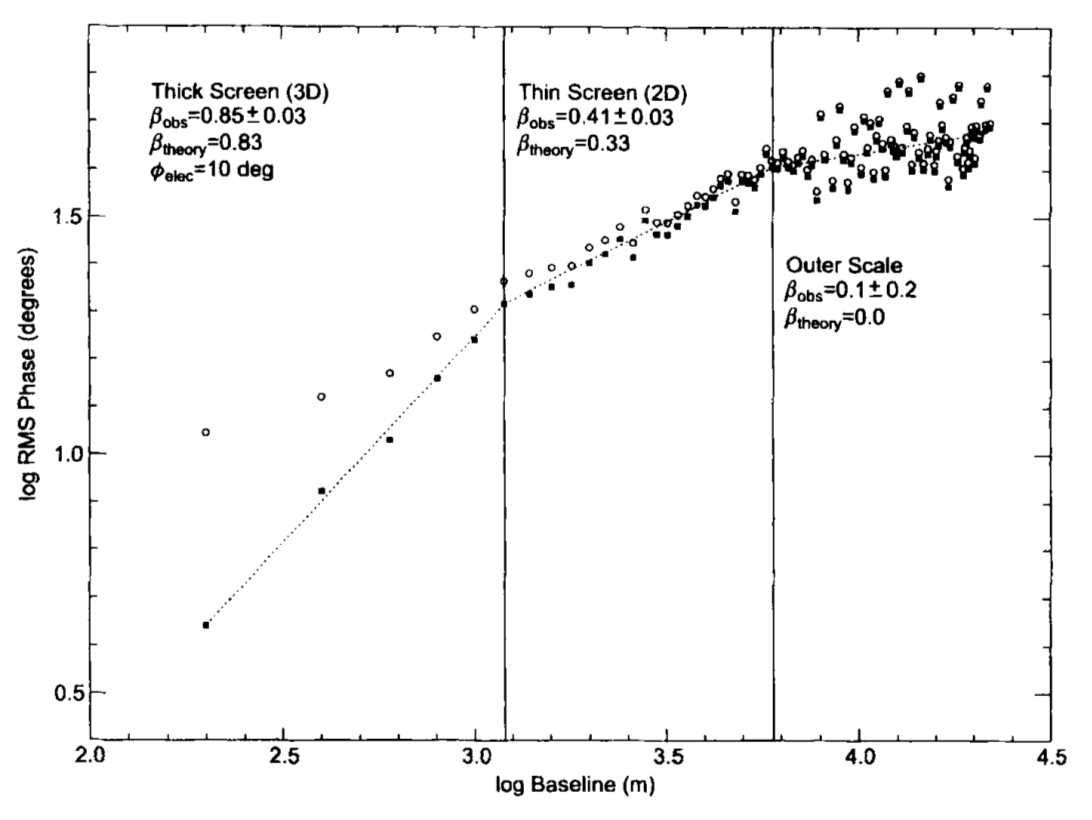
\includegraphics[scale=0.2]{Images/screentransition}
    \caption{showing $\beta$ changes with distance on the phase screen. Note the three distinct regime but continous variation in between}
\end{figure}

\subsection{Instrumental}

\subsubsection{Thermal Noise}
%Pr 1 St 3
%Review the TMS section on thermal noise basics.
%Mild derivation of the thermal noise equation.

Does this properly take into account individual antenna noises that are correlated? Unexpectedly this implementation becomes important for the non-zero trop cp later.

\subsubsection{Antenna Pointing}
%Pr 1 St 2.  Take out implementation
%Intro
All antennas suffer pointing errors to some degree due to a variety of factors including dish flexure due to gravity, wind and thermal loading, as well as drive mechanics. This corresponds to an offset primary beam, which should only translate to minor amplitude errors if the pointing error $\theta_{\rm PE}$ is significantly smaller than the primary beam (i.e. $\theta_{\rm PE} \ll \theta_{\rm PB}$). In the Measurement Equation formalism, this offset can be represented by a modified (shifted) primary beam pattern in the {\bf \it E}-Jones term 
\begin{equation}
{\bf E}_p(l,m) = {\bf E}(l_0 + \delta l_p, m_0 + \delta m_p),
\end{equation}
where $\delta l_p, \delta m_p$ correspond to the directional cosine offsets.
%Motivation, why this could be a problem for mm observations


% Different categories of pointing error i.e. tracking vs slew

We investigate the effect of pointing errors on the 50~m (i.e. fully illuminated) LMT dish configured in an eight station VLBI array. The LMT has been measured to have an absolute pointing accuracy of $\sigma_{\rm abs} = 1-3$~arcsec, where smaller offsets occur when observing sources closer to zenith, and a tracking pointing accuracy $\sigma_{\rm track} < 1$~arcsec \footnote{http://www.lmtgtm.org/telescope/telescope-description/}. We explore the observational effect of these errors through three different pointing error models which explore different instructive and plausible scenarios. The LMT has been singled out as this may well serve as a reference station for the EHT array given its sensitivity and central geographic location. The source used is a circular Gaussian of characteristic size $\Theta_{\rm src}=50$ $\mu$-arcsec, located at the phase centre. For this investigation, as long as $\Theta_{\rm src} \ll \theta_{\rm PB}$, the exact structure of the source is unimportant. We approximate the LMT beam profile using an analytic WSRT beam model \citep{Popping_2008} with a factor of 2 increase in the beam factor $C$ to take into account the increased dish size
\begin{equation}
E(l, m) = \cos^3(C\nu \rho),\qquad   \rho = \sqrt{\delta l_p^2 + \delta m_p^2}
\end{equation}
where $C$ is a constant, with value $C \approx 130$~GHz$^{-1}$. Note that the power beam $EE^H$ becomes $\cos^6$, giving a $\rm{FWHM} = 6.5 $~arcsec. In Fig.~\ref{fig:pointing}, we show this for pointing accuracies spanning the range from $\rho \sim 0-4.5$~arcsec. 

In the first case we assume a constant pointing error and plot the RMS relative visibility amplitude error $\sigma_{\Delta V/V_0}$ on baselines to LMT, where $\Delta V = V_{\rm point} - V_{0}$, $V_{\rm point}$ and $V_{0}$ are the amplitude of the visibility with and without pointing errors respectively. This simulation is meant to be instructive as to the typical amplitude error in the simplest possible scenario.


Also interesting to consider is a slower, continuous time-variable pointing error associated with the tracking error $\sigma_{\rm track}$. Physically this could be attributed to changes in wind, thermal and gravitational loading which all change with telescope pointing direction and over the course of a typical few hour observation. Using the MeqTrees software package, such behaviour has been demonstrated to occur with the Westerbork Synthesis Radio Telescope (WSRT, \cite{Smirnov_2011c})\footnote{See also https://indico.skatelescope.org/event/\\171/session/9/contribution/20}. This is modeled as a sinusoid with period sampled from a uniform distribution between 0.5 and 6 hours, and a peak amplitude $A_{\rho} = \sqrt{2} \sigma_{\rho}$ , where the factor $\sqrt{2}$ relates the amplitude to the RMS for periodic zero mean waveforms. 


Whilst a stationary phase centre is tracked, the pointing error should evolve slowly and smoothly, however, in mm-VLBI observations the phase centre is often shifted to another source/calibrator. This would cause the pointing error to change abruptly, with an absolute pointing error $\sigma_{\rm abs}$. Source/calibrator change is scheduled every 5-10 minutes in a typical millimetre observation. The point is that even though EHT will be able to determine the pointing offset when observing a calibrator with well known structure, when the antennas slew back to a source (e.g. Sgr~A$^\star$) with less certain or variable source structure, the pointing error could change significantly. This is exacerbated by the scarcity of mm-wavelength calibrators, which are often widely separated from the source. We simulate this effect by re-sampling the pointing error every 10 minutes from a Gaussian of characteristic width equal to the quoted pointing error. We perform 50 realisations of the simulation for each pointing offset to generate reasonable uncertainties.




\subsubsection{Polarisation}
% Leave for now



